\subsection{Static Checking}
%Go over the static checking done, explain the errors we pick up on, the various "categories" and how we still split up it into phases.

The static checker is in charge of verifying the validity of the code ensuring that the engine can run it. The phase exists so that the code can be checked thoroughly all at once rather than having the game designer debug errors during runtime. In the JavaScript implementation, this is done during the parse and compile phase. In the design of our Rascal implementation, this is done after the post-processing phase and before the compilation phase\dd. Static code analysis is used to generate human-readable error messages before the compiler transforms the code into more complex Rascal data structures.

The static checker verifies the integrity of each component in a specific order. Components that define variables that can be referenced later are checked as soon as possible so that the references can be checked before they are used. Each component is checked for integrity based on the design extracted from the JavaScript implementation. Because the static checker isolates components errors, code cannot cascade and taint the rest of the file\dd, this is shown in Figure \ref{fig:checker_example}. An error can, at most, make it impossible to check the current component. In those cases, the checker will return the current error message and move on to the next component. The only case in which errors 'spill' is when an invalid component is referenced. In this case, the checker will also generate an error stating that the reference to the invalid component does not exist. This amount of 'spill' is acceptable as it only happens in cases where the component has severe syntax errors.

\begin{figure}[!t]
    \centering
    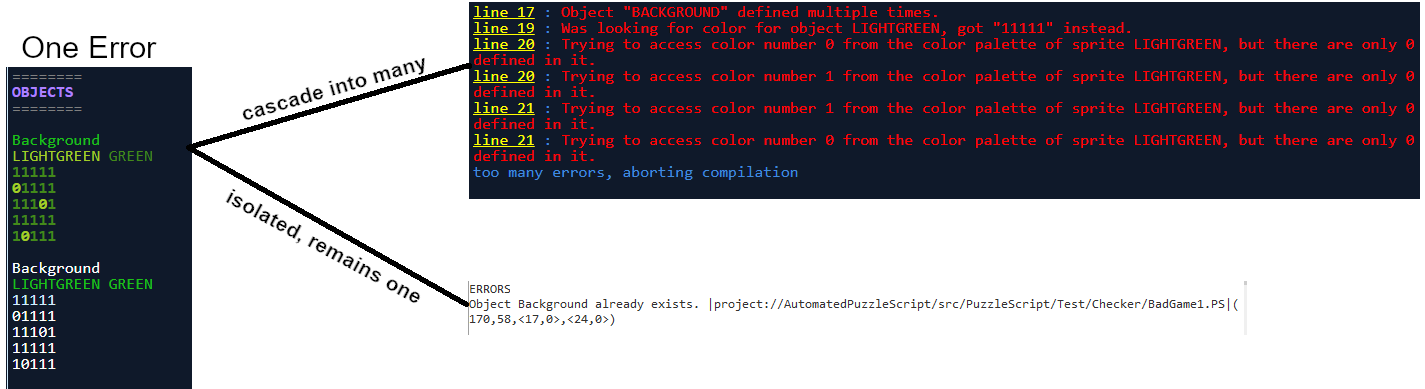
\includegraphics[width=1\textwidth]{images/Example checker.png}
    \caption{Isolation of errors}
    \label{fig:checker_example}
\end{figure}

The JavaScript implementation has 117 unique error/warning messages. This number does not account for messages that appear multiple times. Although our design currently checks for only 72 messages, the discrepancy has two reasons. As previously mentioned, using Rascal's Syntax Definition entails a certain loss of control over the feedback provided in exchange for more readability. The first reason is therefore that a part of these messages are now covered by the general parser failure error intended for the tool designer. The second reason is that, in our design, another part of the messages we extracted from the original implementation have been merged\dd. For instance, the original message has two separate messages to report on an error within the rule depending on whether that error was on the left-hand side or the right-hand side. In our design, these errors are merged into one with a keyword to differentiate the side that raised the error.

\begin{figure}[!t]
    \centering
    \begin{subfigure}{1\textwidth}
        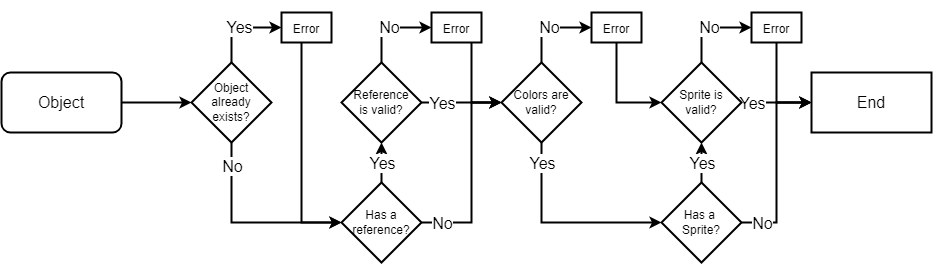
\includegraphics[scale=0.45]{images/checker/Object.png}
        \caption{Flow diagram when validating an Object}
        \label{fig:checker_object}
    \end{subfigure}
    \begin{subfigure}{1\textwidth}
        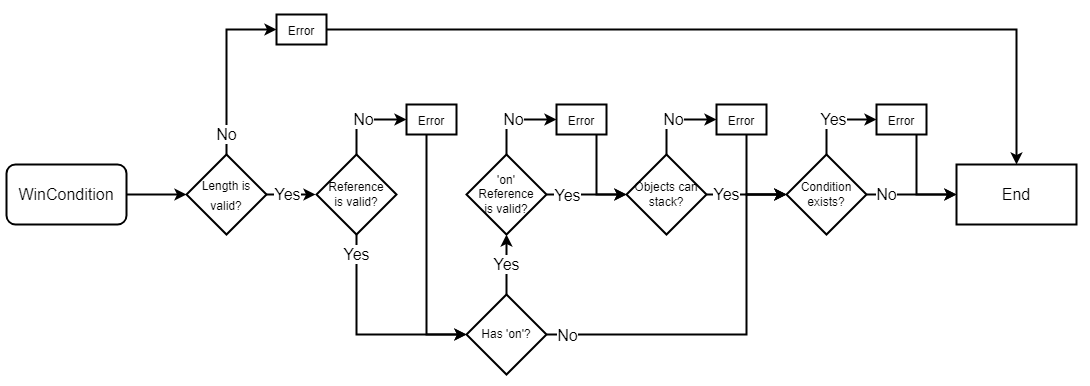
\includegraphics[scale=0.45]{images/checker/WinCondition.png}
        \caption{Flow diagram when validating a WinCondition}
        \label{fig:checker_condition}
    \end{subfigure}
    \caption{Flow diagrams illustrating the validation process done by the checker}
\end{figure}

Figure \ref{fig:checker_object} shows an example of how the checker processes a PuzzleScript component, in this case an Object. Diamonds represent tests that the checker submits the code to and rectangles represent an outcome. This is a simplification of the process that omits specifics on what is considered 'valid'. For instance, a valid color is either a HTML color code or a selection from the color palette selected by the game designer in the prelude. Objects that do not pass the requirement generate an error message that is returned by the checker, to be displayed later. In some cases, an early error causes the remaining checks to be skipped as can be seen in Figure \ref{fig:checker_condition} which illustrates the process for a Win Condition. Figure \ref{fig:checker_remaining} shows how the static checker validates the remaining components of PuzzleScript. Once detected an error is not immediately displayed but rather stored\dd, this serves the dual benefit of making it easy for the IDE to customize how they display the messages and allowing us to centralize our human-readable conversions of these messages. As a result, our redesign is easier to extend in the cases where a tool designers wants to modify the messages. For instance, if a tool designer wants to translate PuzzleScript, all they have to do is go through a single file to have access to the messages. 

In our design, error messages have several different types and subcategories. The main types are \emph{errors} and \emph{warnings}, support for lower categories exist but are currently unused. Generated messages also fall under one of a few sub-categories:
\begin{itemize}
    \item Invalid: The component's syntax is not respected making it unusable
    \item Undefined: The reference/object with that name is never defined but is used
    \item Existing:  The reference/object with that name already exists, but the code is trying to define it again. Sometimes this is generated as an error and sometimes as a warning depending on whether the engine can handle it.
    \item Unused: A warning, the code defines a reference/object/sound but never uses it\dd.
    \item Misc: Very specific errors that do not occur in enough numbers to justify a category
\end{itemize}

We categorize each error with a degree of importance based on whether or not it has a negative impact on the game and its ability to run. Error-level messages can cause issues or unintended side effects in the code that may make the game impossible to resolve, warning-level messages indicate dead or unoptimized code, and information-level messages inform the game designer on gameplay quality and possible best practices. A full list of errors and warnings raised by our tool can be seen in Appendix B. 

\begin{figure}
\vspace*{-4pt}
%\begin{minipage}{0.31\columnwidth}
%\begin{lstlisting}[language=PuzzleScript, xleftmargin=4pt]
%Background
%red green
%11111
%01111
%11101
%11111
%10111
%
%Background
%Red Green
%11111
%01111
%11101
%11111
%10111
%\end{lstlisting}
%\subcaption{duplicate object}
%\end{minipage}
%
%
\begin{minipage}{0.32\columnwidth}
%vRozen: what is Bonk?
\setulcolor{red}
\begin{lstlisting}[language=PuzzleScript, xleftmargin=2pt, , basicstyle=\ttfamily\footnotesize]
Player
black $\color{BurntOrange}orange$ $\color{darkgray}white$ $\color{blue}blue$
$\color{black}.000.$
$\color{black}.$$\color{BurntOrange}111$$\color{black}.$
$\color{darkgray}22222\ul{22222}$
$\color{black}.$$\color{blue}333$$\color{black}.$
$\color{black}.$$\color{blue}3$$\color{black}.$$\color{blue}3$$\color{black}.$
\end{lstlisting}
\setulcolor{black}
% \vspace*{-9.5pt}
\subcaption{Sprite not 5x5}
\setulcolor{black}
\end{minipage}
\hspace{12pt}
%
\begin{minipage}{0.31\columnwidth}
\setulcolor{red}
\begin{lstlisting}[language=PuzzleScript, xleftmargin=4pt,  basicstyle=\ttfamily\footnotesize]
####
#.O#$\ul{..}$
#..#$\ul{\#\#..}$
#@P.$\ul{.\#}$
#..*
#..#$\ul{\#\#}$
####$\ul{..}$
\end{lstlisting}
\subcaption{Uneven level rows}
\setulcolor{black}
\end{minipage}
\hspace{12pt}
\begin{minipage}{0.28\columnwidth}
% \setulcolor{Gold}
\begin{lstlisting}[language=PuzzleScript, xleftmargin=4pt, basicstyle=\ttfamily\footnotesize]
Crate
$\color{BurntOrange}orange$ $\color{Green}\ul{green}$
$\color{BurntOrange}00000$
$\color{BurntOrange}0$$\color{black}...$$\color{BurntOrange}0$
$\color{BurntOrange}0$$\color{black}...$$\color{BurntOrange}0$
$\color{BurntOrange}0$$\color{black}...$$\color{BurntOrange}0$
$\color{BurntOrange}00000$
\end{lstlisting}
\subcaption{Unused color}
\setulcolor{black}
\end{minipage}
\medskip

\begin{minipage}{\columnwidth}
%, xleftmargin=4pt, basicstyle=\ttfamily\scriptsize]
\setulcolor{red}
\begin{lstlisting}[language=PuzzleScript, basicstyle=\ttfamily\footnotesize]
[Eyeball| ... |Player] -> $\ul{[> Eyeball|Player]}$
\end{lstlisting}
\vspace*{-4pt}
\subcaption{Missing ellipsis in right hand side of rule}
\setulcolor{black}
\end{minipage}
\medskip

\begin{minipage}{\columnwidth}
%, xleftmargin=4pt, basicstyle=\ttfamily\scriptsize]
\setulcolor{red}
\begin{lstlisting}[language=PuzzleScript, xleftmargin=10pt, basicstyle=\ttfamily\footnotesize]
[> Player|Crate] -> [> Player] $\ul{[> Crate]}$
\end{lstlisting}
\vspace*{-4pt}
\subcaption{Unexpected rule part in right hand side of rule}
\setulcolor{black}
\end{minipage}

\caption{Errors and warnings detected by the checker}
\label{fig:ErrorsWarnings}
\vspace*{-8pt}
\end{figure}

As we previously mentioned, our tool raises errors and warnings that do not exist in the original implementation. Part of these messages are merges and others are brand news\dd. A sample of these new messages is displayed in Table \ref{tab:new_errors}. Many of these messages reference existing objects that are never used. Unused objects present two issues. The first issue is that unused objects represent dead code that inflate the file size but add no value. Dead code adds unnecessary complexity to the codebase and makes it more difficult to understand. The second issue is that unused objects may also give a false impression of the game. This false impression of the game makes it hard for other game designers to understand the design of the game. Our tool also raises a warning when redundant components are implemented into the game. For instance, duplicate win conditions can happen when game designers are not fully aware of what object a legend references. This can cause them to create duplicate instances through the use of different legends referencing the same item. Finally, ScriptButler performs additional checks on Win Conditions, an area left relatively untouched by the original implementation. We design checks to ensure that game designers do not accidentally write conditions that are mutually exclusive.

\begin{table}
\centering
\caption{New errors in ScriptButler}
\label{tab:new_errors}
\begin{tabular}{l|l|l}
Name                               & Type    & Message                                                                                                                    \\ \hline
existing\_sound                    & Warning & \begin{tabular}[c]{@{}l@{}}A sound event has already been \\ registered for this object with \\ these actions\end{tabular} \\
existing\_condition                & Warning & \begin{tabular}[c]{@{}l@{}}A victory condition similar to \\ this one already exists\end{tabular}                          \\
existing\_rule                     & Warning & \begin{tabular}[c]{@{}l@{}}A rule similar to this one already \\ exists\end{tabular}                                       \\
impossible\_condition\_unstackable & Error   & \begin{tabular}[c]{@{}l@{}}A victory condition requires items \\ existing on the same layer to stack\end{tabular}          \\
redundant\_prelude\_value          & Warning & \begin{tabular}[c]{@{}l@{}}This prelude keyword does not \\ require a value\end{tabular}                                   \\
unused\_colors                     & Warning & \begin{tabular}[c]{@{}l@{}}This object defines more colors \\ than it uses\end{tabular}                                    \\
unused\_object                     & Warning & This object is defined but never used                                                                                      \\
unused\_legend                     & Warning & This legend is defined but never used                                                                                     
\end{tabular}
\end{table}

The result of this phase is a list of messages reporting on the state of the game's code. The intent is for those messages to be passed on to the IDE and displayed to the user as shown in \ref{fig:ErrorsWarnings}. The game designer gains a complete overview of the game code and an understanding of its current flaws. Once the designer has resolved the errors, the game code is passed to he compiler. The compiler is discussed in the next section.

